\documentclass{article}
\usepackage[UTF8]{ctex}
\usepackage{underscore}
\usepackage{enumerate}
\usepackage{graphicx}
\title{Algorithm Design and Analysis}
\date{Assignment 1}
\author{吴长亮}
\begin{document}
\maketitle

\section{Question 1}
\subsection{Algorithm Description}
  \subsubsection{Description}

  \begin{itemize}
  \item 分别找到两个数组的n/2位置的中位数M1,M2
  \item 比较M1、M2大小,去掉每个数组一半的数据
  \item 递归执行比较
  \end{itemize}

  \subsubsection{Pseudo-code}

  \begin{enumerate}[1:]
  \item find_mid($l_{1}$,$r_{1}$,$l_{2}$,$r_{2}$)
  \item if $l_{1}$==$r_{1}$ then
  \item   return ($l_{1}$+$l_{2}$)/2
  \item end if
  \item M1=array1_mid
  \item M2=array2_mid
  \item if $M1<M2$ then
  \item   find_mid(array1_mid,$r_{1}$,$l_{2}$,array2_mid)
  \item else
  \item   find_mid($l_{1}$,array1_mid,array2_mid,$r_{2}$)
  \item end if
  \end{enumerate}

\subsection{Subproblem Reduction Graph}
  \centerline{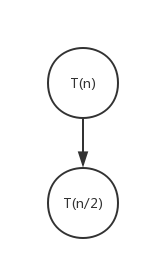
\includegraphics[scale=0.6]{q1.png}}

\subsection{Correctness}
中点划分中位数,包含所有的数据

\subsection{Complexity}
  $$ T(n) = T(n/2) + c $$
所以复杂度为$O(log_n)$

\section{Question 2}
\subsection{Algorithm Description}
  \subsubsection{Description}
  \begin{itemize}
  \item 二叉树的最长路径:1.左子树的最长路径2.右子树的最长路径3.左子树的高度加右子树的高度
  \item 分别递归左右子树
  \item 计算节点高度
  \item 左子树的最大长度,右子树的最大长度,左子树的最大深度+右子树的最大深度,取三者的最大值就是当前节点的最长路径
  \end{itemize}

  \subsubsection{Pseudo-code}
  \begin{enumerate}[1:]
  \item max_dis(root)
  \item if 叶子节点 than
  \item   return
  \item left=max_dis(左节点)
  \item right=max_dis(右节点)
  \item max=max(左子树高度,右子树高度)
  \item return max(左子树的最大长度,右子树的最大长度,左子树的最大深度+右子树的最大深度+2)
  \end{enumerate}

\subsection{Subproblem Reduction Graph}
  \centerline{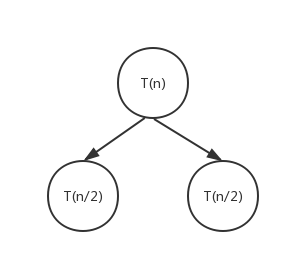
\includegraphics[scale=0.6]{q2.png}}
\subsection{Correctness}
子树递归调用遍历所有的节点
\subsection{Complexity}
  $$ T(n) = 2T(n/2) + c $$
  所以复杂度为$O(n)$
\section{Question 3}
\subsection{Algorithm Description}
  \subsubsection{Description}
  \begin{itemize}
    \item 根节点符合
    \item 取左右子树较小的树,必有极小值
    \end{itemize}
  \subsubsection{Pseudo-code}
  \begin{enumerate}[1:]
    \item local_min(root)
    \item if 根节点最小
    \item return
    \item local_min(min(root$->$left,root$->$right))
  \end{enumerate}
\subsection{Subproblem Reduction Graph}
  \centerline{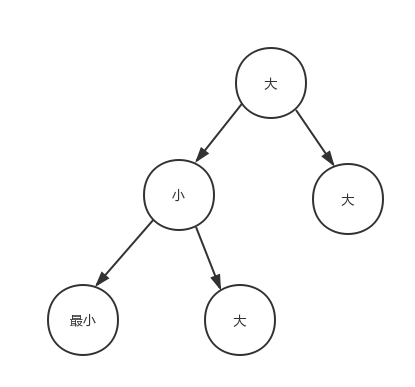
\includegraphics[scale=0.6]{q3.png}}
\subsection{Correctness}
取较小值之后,如果左右子树大,那么该节点就最小,否则走到叶子节点就是最小
\subsection{Complexity}
最坏情况走到叶子节点,复杂度为树高,即$O(log_n)$
\end{document}
